%!TEX root = ComputerScienceOne.tex

\label{chapter:functions}

%Introduction/Motivation

In mathematics, a function is a mapping from a set of \emph{inputs}
to a set of \emph{outputs} such that each input is mapped to exactly one
output.  For example, the function 
  $$f(x) = x^2$$
maps numeric values to their squares.  The input is a variable $x$.  When
we assign an actual value to $x$ and evaluate the function, then the function
has a value, its output.  For example, setting $x = 2$ as input, the output
would be $2^2 = 4$.  Mathematical functions can have multiple inputs, 
  $$f(x,y) = x^2 + y^2 \quad f(x, y, z) = 2x + 3y - 4z$$
However, a function will only ever have a single output value.

In programming languages, a \gls{function} (sometimes called subroutine 
or procedure) can take multiple inputs and produce one output value.  We've 
already seen some examples of these functions.  For example, most languages 
provide a math library that you can use to evaluate the square root or 
sine of a value $x$.  We've also seen some functions with multiple input 
values such as the ``power'' function that allows you to compute $f(x, y) = x^y$.
Finally, the main entry point to many programs is defined by a main function.

More formally, a function is a sequence of instructions (code) that is 
packaged into a \emph{unit} that can be reused.  A function performs 
a specific task: given a number of inputs, it executes some sequence 
of operations (executes some code) and ``returns'' (outputs) a result.
The output can be captured into a variable or used in an expression by 
whatever code \emph{invoked} or ``called'' the function.

Defining and using functions in programming has numerous advantages.
The most obvious advantage is that it allows you a way to \emph{organize} 
code.  By separating a program it into distinct units of code it is more organized 
and it is clearer what each piece or segment of code does.  This also 
facilitates \index{top-down design} \gls{top-down design}: one way to approach a problem is to 
split it up into a series of subproblems until each subproblem is either trivial 
to deal  with, or an existing, ``off-the-shelf'' solution already exists for it.
Functions may serve as the logical unit for each subproblem.  

Another advantage is that by organizing code into functions, those functions 
can be \emph{reused} in multiple places either in your program/project 
or even in other programs/projects.  A prime example of this are the standard
libraries available in most programming languages that provide functions
to perform standard input/output or mathematical functions.  These standard
libraries provide functions that are used by thousands of different programs
across multiple different platforms.

Functions also form an \emph{isolated} unit of code.  This allows for 
better and easier \emph{testing}.  By isolating pieces of code, we can 
rigorously test those pieces of code by themselves without worrying 
about the larger program or contexts.  

Functions facilitates \index{procedural abstraction} 
\gls{procedural abstraction}.  Placing code 
into functions allows you to abstract the details of how the function computes 
its answer.  As an example: consider a standard math library's square root
function: it may use some interpolation method, a Taylor series, or some 
other method entirely to compute the square root of a given number.  
However, by putting this functionality into a function, we, as programmers, 
do not need to concern ourselves about these details.  Instead, we simply 
\emph{use} the function, allowing us to focus on the larger issues at hand 
in our program.

\section{Defining \& Using Functions}

Like variables, many programming languages may require that you declare a 
function before you can use it.  A function
declaration may simply include a description of the function's input/output
and name.  A function declaration may require you to define
the function's body at the same time or separately.  Functions can also
have \index{scope} scope: some areas of the code may be able to ``see'' the function
or know about it and be able to invoke the function while other areas of
the code may \emph{not} be able to see the function and therefore may
not be able to invoke it.  

Some interpreted programming languages use function \index{hoisting} \gls{hoisting} which allows
you to use/invoke functions \emph{before} you declare them.  This works
because the interpreter does an initial scan of the code and
identifies all function declarations.  Only after it has ``hoisted'' all functions
into scope does it start to execute the program.  Thus, a function declaration
can appear \emph{after} it has been used and it will still work.

\subsection{Function Signatures}

A function is usually defined by its \gls{signature}: every function can be
identified by its name (also called an \emph{identifier}), its list of 
\emph{input parameters}, and its \emph{output}.  A function signature
allows the programming language to uniquely identify each function
so that when you invoke a function there is no ambiguity in which function
you are calling.

\begin{algorithm}[H]
\Fn{sum(a, b)}{
  $x \leftarrow a + b$ \;
  return $x$ \;
}
\caption[A function in pseudocode]{A function in pseudocode.  In this case, the name (identifier) of
the function is \emph{sum} and it has two parameters, $a$ and $b$.  Its
body is contained in lines 2--3.  Its return value is indicated by the return
statement on line 3.}
\label{algorithm:function}
\end{algorithm}

A function declaration in pseudocode is presented in Algorithm 
\ref{algorithm:function}.  In the pseudocode, explicit variable types
are omitted, and thus the return type is inferred from the return statement.
In Figure \ref{figure:cFunctionPrototype} we have provided an example
of a function declaration in the C programming language with each
element labeled. 

\begin{figure}[!h]
\centering
%\documentclass[12pt]{article}
%\usepackage{tikz}
%\usetikzlibrary{backgrounds}
%\usetikzlibrary{decorations.pathreplacing}
%
%%\usepackage{newfloat}
%\usepackage{minted}
%\setminted{mathescape,
%               linenos,
%               autogobble,
%               frame=none,
%               framesep=2mm,
%               framerule=0.4pt,
%               %label=foo,
%               xleftmargin=2em,
%               xrightmargin=0em,
%               numbersep=10pt, %gap between line numbers and start of line
%               style=default}
%\usepackage{fullpage}
%\begin{document}

\begin{tikzpicture}[framed]

  \node (main) {
{
\mintinline[]{c}{double getDistance(double x1, double y1, double x2, double y2);}
}
  
  };

%  \node (formatstring) at (-5,2) {Format String};

%  \node (placeholders) at (1,-1.5) {Placeholders};
 % \draw[->] (placeholders.north) -- ([xshift=-.70cm,yshift=0.15cm]main.south);
  %\draw[->] (placeholders.north) -- ([xshift=3.7cm,yshift=0.2cm]main.south);
  
  \draw [decorate,decoration={brace,amplitude=10pt},xshift=-4pt,yshift=0pt] ([xshift=-2.65cm]main.north) -- ([xshift=6.25cm]main.north) node [black,midway,yshift=0.65cm] {Parameters};

  \draw [decorate,decoration={brace,mirror,amplitude=5pt},xshift=-4pt,yshift=0pt] ([xshift=-6.75cm]main.south) -- ([xshift=-5.5cm]main.south) node [below,align=center,text width=2cm,black,midway,yshift=-0.25cm] {Return Type};

  \draw [decorate,decoration={brace,mirror,amplitude=5pt},xshift=-4pt,yshift=0pt] ([xshift=-5.25cm]main.south) -- ([xshift=-3.0cm]main.south) node [below,align=center,text width=2cm,black,midway,yshift=-0.25cm] {Identifier (name)};

%\draw[black,fill=black] (placeholders.north) circle (.5pt);

\end{tikzpicture}

%\end{document}

\caption{A function declaration (prototype) in the C programming language
with the return type, identifier, and parameter list labeled.}
\label{figure:cFunctionPrototype}
\end{figure}

Some languages only allow you to use one identifier for one function 
(like variables) while other languages allow you to define multiple functions
with the same identifier as long as the parameter list is different (see
Section \ref{subsection:functionOverloading} below).  In general, like variables, function names
are case sensitive.  Also similar to variables, modern lower camel casing
is used with function names.  

When defining the parameters to a function (its input), you usually provide
a comma delimited list of variable names.  In the case of statically typed
languages, the types of the variable parameters are also specified.  The
order is important as when you invoke the function, the number of inputs
must match the number of parameters in the function declaration.  The 
variable types may also need to match.  In some dynamically typed languages, 
you may be able to call functions with different types or you may be able
to omit some of the parameters (see Section \ref{subsection:optionalParameters}
below).

Similarly, the return type of the function may need to be specified in 
statically typed languages while with dynamic languages, functions may
conditionally return different types.  We generally refer to the ``return value''
or ``return type'' because when a function is done executing, it ``returns''
the control flow back to the line of code that invoked it, returning its
computed value.

You can also define functions that may not have any inputs or may not
have any output.  Some languages use the keyword \mintinline{text}{void} 
to indicate no return value and such functions are known as ``void 
functions.''  When a function doesn't have any input values, its parameter
list is usually empty.

The function signature may be accompanied by the function \emph{body}
which contains the actual code that specifies what the function does.  
Typically the function body is demarcated with a code block using 
opening and closing curly brackets, \mintinline{text}{{ ... }}.  Within the function you can generally
write any valid code including declaring variables.  When you declare a 
variable inside a function, however, it is \index{scope!local} \emph{local} to that function.
That is, the variable's scope is only defined within the function.  A local
variable cannot be accessed outside the function, indeed the local
variable does not usually survive when the function ends its
execution and returns control back to line of code that called it. 
Function parameters are essentially locally scoped variables as well 
and can usually be treated as such.

\subsection{Calling Functions}
\index{invoking functions}
\index{calling functions|see {invoking functions}}

When a function has been defined and is in scope, you can \emph{invoke}
or ``call'' the function by coding the function name and providing the input
parameters which can be either variables or literals.  When
provided as inputs, parameters are referred to as \emph{arguments}
to the function.  The arguments are typically provided as a comma delimited
list and placed inside parentheses.  

Invoking a function changes the usual flow of control.  When invoked, control
flow is transferred over to the function.  When the function finishes executing the
code in its body, control flow returns to the point in the code that invoked it.
It is common for a program to be written so that a function calls another function
and that function calls another.  This can form a deep chain of function calls in 
which the flow of control is transferred multiple times.  Upon the completion
of each function, control is returned back to the function that called it, 
referred to as the \emph{calling function}.

If a function returns a value it can either be captured in a variable using an
assignment operator or by using it in an expression.  

\begin{algorithm}[H]
$a \leftarrow 10$ \;
$b \leftarrow 20$ \;
$c \leftarrow sum(a, b)$ \;
\caption[Using a function]{Using a function.  We invoke a function by 
indicating its name (identifier) and passing it arguments.}
\label{algorithm:functionCall}
\end{algorithm}

\subsection{Organizing}   

Functions provide code organization, but functions themselves should also
be organized.  We've seen this with standard libraries.  Functions that provide
basic input/output are all grouped together into one library.  
Functions that involve math functions are grouped together into a separate math library.

Some languages allow you to define and ``import'' individual libraries 
which organize similar functions together.  Some languages do this by 
collecting functions into ``utility'' classes or \emph{modules}.  Only when
you import these modules do the functions come into scope and can be
used in your code.  If you do not import these modules, then the functions
are out of scope and cannot be used.  

In some languages once a function is imported it is part of the 
\index{global scope|see {scope!global}} \index{scope!global}
\emph{global scope} and can be ``seen'' by any part of the code.  This can cause
\emph{conflicts}: if you import modules from two different libraries each
with different functions that have the same name or signature, then 
the two function definitions may be in conflict or it may make your
code ambiguous as to which function you intend to invoke.  This is
sometimes referred to as ``polluting the namespace.''  There are
several techniques that can avoid this situation.  Some languages allow
you to place functions into a \emph{namespace} to keep functions with
the same name in different ``spaces.''  Other languages allow you to 
place functions into different classes and then invoke them by explicitly
specifying \emph{which} class's function you want to call.  Yet other
languages don't have great support for function organization and it is
the library designer's responsibility to avoid naming conflicts, typically
by adding a library-specific prefix to every function.

\section{How Functions Work}
\label{section:howFunctionsWork}

To understand how functions work in practice, it is necessary to 
understand how a program operates at a lower level.  In particular,
each program has a \index{program stack} 
\gls{program stack} (also called a call stack).  
A \gls{stack} is a data structure that holds elements in a \gls{lifoLabel}
manner.  Elements are added to the ``top'' of the stack in an operation
called \emph{push} and elements can be removed from the top
of the stack in an operation called \emph{pop}.  In general, elements 
cannot be inserted or removed from the middle or ``bottom'' of the 
stack.

In the context of a program, a call stack is used to keep track of the 
flow of control.  Depending on the operating system, compiler and architecture, 
the details of how elements are stored in the program stack may 
vary.  In general when a program begins, the operating 
system loads it into memory at the bottom of the call stack.  Global 
variables (static data) are stored on top of the main program.  Each
time a function is called, a new \emph{stack frame} is created and
pushed on
top of the stack.  This frame contains enough space to hold values
for the arguments passed to the function, local variables declared
and used by the function, as well as a space for a return value and
a return \emph{address}.  The return address is a memory location
that the program should return to after the execution of the function.
That way, when the function finishes its execution, the stack frame
can be removed (popped) and the lower stack frame of the calling
function is preserved.  This is a very efficient way to keep track of
the flow of control in a program.  As each function calls 
another function, each stack frame is preserved by pushing a new
one on top of the program stack.  Each time a function terminates execution and returns, the removal
of the stack frame means that all local variables go \emph{out of
scope}.  Thus, variables that are local to a function are not accessible
outside the function.

To illustrate, consider the following snippet of C code.  The \mintinline{c}{main()}
function invokes the \mintinline{c}{average()} function which in 
turn invokes the \mintinline{c}{sum()} function.  Each invocation 
creates a new stack frame on top of the last in the program stack
which is depicted in Figure \ref{figure:programStack}.

\begin{minted}{c}
double sum(double a, double b) {
  double x = a + b;
  return x;
}

double average(double a, double b) {
  double y = sum(a, b) / 2.0;
  return y;
}

int main(int argc, char **argv) {
  double n = 10.0;
  double m = 16.0;
  double ave = average(n, m);
  printf("average = %f\n", ave);
  return 0;
}
\end{minted}

\begin{figure}[!h]
\centering
%\documentclass[12pt]{article}
%\usepackage{tikz}
%\usepackage{minted}
%\usetikzlibrary{decorations.pathreplacing}
%\usetikzlibrary{fadings}
%\usepackage{fullpage}
%\begin{document}
%\begin{figure}
%\centering

\begin{tikzpicture}[auto,scale=0.80,transform shape,every node/.style={text centered, text width=5.5cm}]

\node [above left] (bottom) at (0,0) {Bottom of the stack (high memory)};
\node [below left] (top) at (0,15.5) {Top of the stack (low memory)};

\draw (6,18.5) -- (6, 15.5);
\draw[path fading=north] (0,15.5) -- (0, 18.5);
\node [above] (unused) at (3, 16) {Unused stack space};

\draw[fill=blue!10!white] (0, 0) rectangle (6,2);
\node [above] (pc) at (3,0) {Program Code};

\draw[fill=yellow!10!white] (0, 2) rectangle (6,3.5);
\node [above] (globals) at (3,2) {Global Variables \\ Static Content};

\draw[fill=green!30!white] (0, 3.5) rectangle (6,7.5);
\node [above] (main) at (3,3.5) {arguments \mintinline{c}{argc, argv}};
\draw[dashed] (0, 5) -- (6, 5);
\node [above] (mainvar) at (3,5) {return address, value (\mintinline{c}{0})};
\draw[dashed] (0, 6) -- (6, 6);
\node [above] (mainvar2) at (3,6) {local variables \mintinline{c}{n, m, ave}};
\draw [decorate,decoration={brace,amplitude=10pt,mirror},xshift=4pt,yshift=0pt] (6, 3.5) -- (6, 6.5+1) node [align=left,black,midway,xshift=6.25cm]  {\texttt{main()} stack frame};


\draw[fill=green!20!white] (0, 3.5+4) rectangle (6,7.5+4);
\node [above] (main) at (3,3.5+4) {arguments \mintinline{c}{a, b}};
\draw[dashed] (0, 5+4) -- (6, 5+4);
\node [above] (mainvar) at (3,5+4) {return address, value (\mintinline{c}{12.5})};
\draw[dashed] (0, 6+4) -- (6, 6+4);
\node [above] (mainvar2) at (3,6+4) {local variables \mintinline{c}{y}};
\draw [decorate,decoration={brace,amplitude=10pt,mirror},xshift=4pt,yshift=0pt] (6, 3.5+4) -- (6, 7.5+4) node [align=left,black,midway,xshift=6.25cm]  {\texttt{average()} stack frame};


\draw[fill=green!10!white] (0, 3.5+8) rectangle (6,7.5+8);
\node [above] (main) at (3,3.5+8) {arguments \mintinline{c}{a, b}};
\draw[dashed] (0, 5+8) -- (6, 5+8);
\node [above] (mainvar) at (3,5+8) {return address, value (\mintinline{c}{26.0})};
\draw[dashed] (0, 6+8) -- (6, 6+8);
\node [above] (mainvar2) at (3,6+8) {local variables \mintinline{c}{x}};
\draw [decorate,decoration={brace,amplitude=10pt,mirror},xshift=4pt,yshift=0pt] (6, 3.6+8) -- (6, 7.6+8) node [align=left,black,midway,xshift=6.25cm]  {\texttt{sum()} stack frame};


\end{tikzpicture}


%\end{document}


\caption[Program Stack]{Program Stack.  At the bottom we have the program's code, followed by
static content such as global variables.  Each function call has its own stack frame along with
its own arguments and local variables.  In particular, the variable arguments \mintinline{c}{a} and
\mintinline{c}{b} in two different stack frames are completely different variables.  Upon returning
from the \mintinline{c}{sum()} function call, the top-most stack frame would be popped and removed, 
returning to the code for the \mintinline{c}{average()} function via the return address.
The stack is depicted bottom-up with high memory at the bottom and low memory at the
top, but this may differ depending on the architecture.}
\label{figure:programStack}
\end{figure}


%Recall that everything in a program is stored in memory; variables, 
%constants, values, etc.  Of course, this \emph{includes} the program
%itself.  Each function in a program is stored at some memory address

\subsection{Call By Value}
\index{call by value}

When a function is invoked, arguments are passed to it.  When you
invoke a function you can pass it variables as arguments.  However, the
variables themselves are not passed to the function, but instead the
values \emph{stored} in the variables at the time that you call the
function are passed to the function.  This mechanism is known as 
\gls{call by value} and the variable values are \emph{passed by value}
to the function.

Recall that the arguments passed to a function are placed in a new
stack frame for that function.  Thus, in reality \emph{copies} of the
values of the variables are passed to the function.  Any changes to
the parameters inside the function have \emph{no effect} on the
original variables that were ``passed'' to the function when it was 
invoked.  

%(TODO: is there a more pseudocody way of doing this?)
To illustrate, consider the following C code.  We have a function \mintinline{c}{sum}
that takes two integer parameters \mintinline{c}{a} and \mintinline{c}{b}
which are passed by value.  Inside \mintinline{c}{sum}, we create another
variable \mintinline{c}{x} which is the sum of the two passed variables.
We then \emph{change} the value of the first variable, \mintinline{c}{a}
to \mintinline{c}{10}.  Elsewhere in the code we call \mintinline{c}{sum}
on two variables, \mintinline{c}{n}, \mintinline{c}{m} with values
5 and 15 respectively.  The invocation of the function \mintinline{c}{sum} 
means that the two values, 5 and 15, stored in the variables are
copied into a new stack frame.  Thus, changing the value to the
first parameter \emph{changes the copy} and has no effect on the
variable \mintinline{c}{n}.  At the end of this code snippet \mintinline{c}{n}
retains its original value of 5.  The program stack frames are depicted
in Figure \ref{figure:PassByValue}.

\begin{minted}{c}
int sum(int a, int b) {
  int x = a + b;
  a = 10;
  return x;
}

...

int n = 5;
int m = 15;
int k = sum(n, m);
\end{minted}

%\documentclass[12pt]{scrbook}
%
%\usepackage{tikz}
%\usepackage{minted}
%\usetikzlibrary{decorations.pathreplacing}
%\usetikzlibrary{patterns}
%
%\usepackage{fullpage}
%\usepackage{subfigure}
%\begin{document}
%
%
%Lorem Ipsum is simply dummy text of the printing and typesetting industry. Lorem Ipsum has been the industry's standard dummy text ever since the 1500s, when an unknown printer took a galley of type and scrambled it to make a type specimen book. It has survived not only five centuries, but also the leap into electronic typesetting, remaining essentially unchanged. It was popularised in the 1960s with the release of Letraset sheets containing Lorem Ipsum passages, and more recently with desktop publishing software like Aldus PageMaker including versions of Lorem Ipsum.
%

\begin{figure}
\centering

\subfigure[Upon invocation of the \mintinline{c}{sum()} function, a new stack frame is created which holds
the parameters and local variable.  The parameter variables \mintinline{c}{a} and \mintinline{c}{b}
are \emph{distinct} from the original argument variables \mintinline{c}{n} and \mintinline{c}{m}.]{

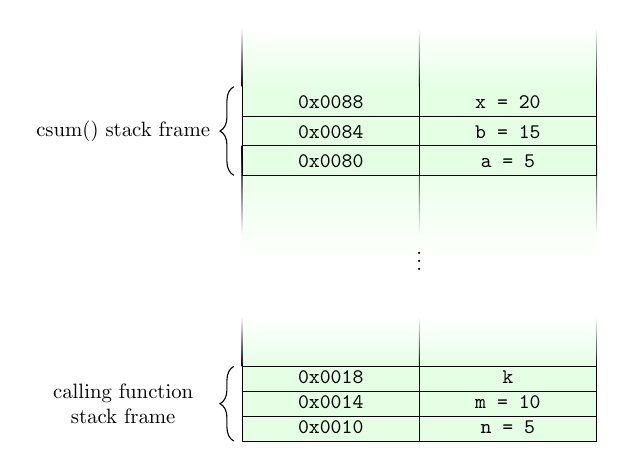
\begin{tikzpicture}[auto,scale=.75,transform shape,every node/.style={text centered}]

%\draw[path fading=north] (0,15.5) -- (0, 18.5);

\draw[fill=green!10!white] (0, 0) rectangle (3, 1.2em);
\node [above] (a1) at (1.5,0) {\texttt{0x0010}};
\draw[fill=green!10!white] (3, 0) rectangle (6, 1.2em);
\node [above] (a2) at (4.5,0) {\texttt{n = 5}};

\draw[fill=green!10!white] (0, 0+1.2em) rectangle (3, 2.4em);
\node [above] (b1) at (1.5,0+1.2em) {\texttt{0x0014}};
\draw[fill=green!10!white] (3, 0+1.2em) rectangle (6, 2.4em);
\node [above] (b2) at (4.5,0+1.2em) {\texttt{m = 10}};

\draw[fill=green!10!white] (0, 0+2.4em) rectangle (3, 3.6em);
\node [above] (b1) at (1.5,0+2.4em) {\texttt{0x0018}};
\draw[fill=green!10!white] (3, 0+2.4em) rectangle (6, 3.6em);
\node [above] (b2) at (4.5,0+2.4em) {\texttt{k}};

\path [top color=white, bottom color=green!10!white] (0,3.625em) rectangle (6,6em);

\fill [top color=white, bottom color=black] (-0.0075,3.6em) rectangle (.02em,6em);
\fill [top color=white, bottom color=black] (5.9925,3.6em) rectangle (6.0075,6em);
\fill [top color=white, bottom color=black] (2.9925,3.6em) rectangle (3.0075,6em);
      
%\draw[top color=white,
%      bottom color=green!10!white]
% (0,3.6em) rectangle (6,6em);
 
%\draw[bottom color=transparent!0,top color=transparent!100] (0,3.6em) -- (0,6em);
%\draw[] (6cm,3.6em) -- (6cm,6em);

%\draw[dashed] (0, 5) -- (6, 5);
%\node [above] (mainvar) at (3,5) {return address, value (\mintinline{c}{0})};
%\draw[dashed] (0, 6) -- (6, 6);
%\node [above] (mainvar2) at (3,6) {local variables \mintinline{c}{n, m, ave}};
\draw [decorate,decoration={brace,amplitude=5pt},xshift=-4pt,yshift=0pt] (0, 0) -- (0, 3.6em) node [text width=3cm,align=center,black,midway,xshift=-.25cm]  {calling function stack frame};


\path [top color=green!10!white, bottom color=white] (0,3) rectangle (6,5);
\fill [top color=black, bottom color=white] (-0.0075,3.5) rectangle (.01,5);
\fill [top color=black, bottom color=white] (2.9925,3.5) rectangle (3.01,5);
\fill [top color=black, bottom color=white] (5.9925,3.5) rectangle (6.01,5);

\draw[fill=green!10!white] (0, 4.5) rectangle (3, 5);
\node [above] (aa1) at (1.5,4.5) {\texttt{0x0080}};
\draw[fill=green!10!white] (3, 4.5) rectangle (6, 5);
\node [above] (aa2) at (4.5,4.5) {\texttt{a = 5}};

\draw[fill=green!10!white] (0, 5) rectangle (3, 5.5);
\node [above] (bb1) at (1.5,5) {\texttt{0x0084}};
\draw[fill=green!10!white] (3, 5) rectangle (6, 5.5);
\node [above] (bb2) at (4.5,5) {\texttt{b = 15}};

\draw[fill=green!10!white] (0, 5.5) rectangle (3, 6);
\node [above] (cc1) at (1.5,5.5) {\texttt{0x0088}};
\draw[fill=green!10!white] (3, 5.5) rectangle (6, 6);
\node [above] (cc2) at (4.5,5.5) {\texttt{x = 20}};

\draw [decorate,decoration={brace,amplitude=5pt},xshift=-4pt,yshift=0pt] (0, 4.5) -- (0, 6) node [text width=3cm,align=center,black,midway,xshift=-.25cm]  {\mintinline{c}{sum()} stack frame};

\node (dots) at (3, 3.15) {$\vdots$};

\path [top color=white, bottom color=green!10!white] (0,6.01) rectangle (6,7);

\fill [top color=white, bottom color=black] (-0.00725,6) rectangle (.0075,7);
\fill [top color=white, bottom color=black] (5.9925,6) rectangle (6.0075,7);
\fill [top color=white, bottom color=black] (2.9925,6) rectangle (3.0075,7);


\end{tikzpicture}
}~~~~\subfigure[The change to the variable \mintinline{c}{a} in the \mintinline{c}{sum()}
function changes the parameter variable, but the original variable \mintinline{c}{n}
is unaffected.]{

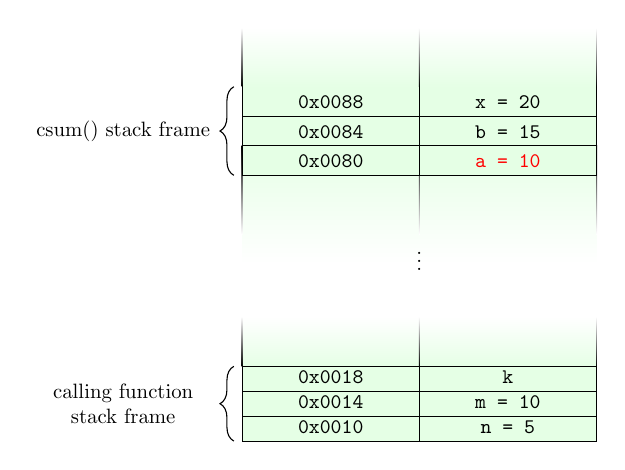
\begin{tikzpicture}[auto,scale=.75,transform shape,every node/.style={text centered}]

%\draw[path fading=north] (0,15.5) -- (0, 18.5);

\draw[fill=green!10!white] (0, 0) rectangle (3, 1.2em);
\node [above] (a1) at (1.5,0) {\texttt{0x0010}};
\draw[fill=green!10!white] (3, 0) rectangle (6, 1.2em);
\node [above] (a2) at (4.5,0) {\texttt{n = 5}};

\draw[fill=green!10!white] (0, 0+1.2em) rectangle (3, 2.4em);
\node [above] (b1) at (1.5,0+1.2em) {\texttt{0x0014}};
\draw[fill=green!10!white] (3, 0+1.2em) rectangle (6, 2.4em);
\node [above] (b2) at (4.5,0+1.2em) {\texttt{m = 10}};

\draw[fill=green!10!white] (0, 0+2.4em) rectangle (3, 3.6em);
\node [above] (b1) at (1.5,0+2.4em) {\texttt{0x0018}};
\draw[fill=green!10!white] (3, 0+2.4em) rectangle (6, 3.6em);
\node [above] (b2) at (4.5,0+2.4em) {\texttt{k}};

\path [top color=white, bottom color=green!10!white] (0,3.625em) rectangle (6,6em);

\fill [top color=white, bottom color=black] (-0.0075,3.6em) rectangle (.02em,6em);
\fill [top color=white, bottom color=black] (5.9925,3.6em) rectangle (6.0075,6em);
\fill [top color=white, bottom color=black] (2.9925,3.6em) rectangle (3.0075,6em);
      
%\draw[top color=white,
%      bottom color=green!10!white]
% (0,3.6em) rectangle (6,6em);
 
%\draw[bottom color=transparent!0,top color=transparent!100] (0,3.6em) -- (0,6em);
%\draw[] (6cm,3.6em) -- (6cm,6em);

%\draw[dashed] (0, 5) -- (6, 5);
%\node [above] (mainvar) at (3,5) {return address, value (\mintinline{c}{0})};
%\draw[dashed] (0, 6) -- (6, 6);
%\node [above] (mainvar2) at (3,6) {local variables \mintinline{c}{n, m, ave}};
\draw [decorate,decoration={brace,amplitude=5pt},xshift=-4pt,yshift=0pt] (0, 0) -- (0, 3.6em) node [text width=3cm,align=center,black,midway,xshift=-.25cm]  {calling function stack frame};


\path [top color=green!10!white, bottom color=white] (0,3) rectangle (6,5);
\fill [top color=black, bottom color=white] (-0.0075,3.5) rectangle (.01,5);
\fill [top color=black, bottom color=white] (2.9925,3.5) rectangle (3.01,5);
\fill [top color=black, bottom color=white] (5.9925,3.5) rectangle (6.01,5);

\draw[fill=green!10!white] (0, 4.5) rectangle (3, 5);
\node [above] (aa1) at (1.5,4.5) {\texttt{0x0080}};
\draw[fill=green!10!white] (3, 4.5) rectangle (6, 5);
\node [above] (aa2) at (4.5,4.5) { \color{red}{\texttt{a = 10}}};

\draw[fill=green!10!white] (0, 5) rectangle (3, 5.5);
\node [above] (bb1) at (1.5,5) {\texttt{0x0084}};
\draw[fill=green!10!white] (3, 5) rectangle (6, 5.5);
\node [above] (bb2) at (4.5,5) {\texttt{b = 15}};

\draw[fill=green!10!white] (0, 5.5) rectangle (3, 6);
\node [above] (cc1) at (1.5,5.5) {\texttt{0x0088}};
\draw[fill=green!10!white] (3, 5.5) rectangle (6, 6);
\node [above] (cc2) at (4.5,5.5) {\texttt{x = 20}};

\draw [decorate,decoration={brace,amplitude=5pt},xshift=-4pt,yshift=0pt] (0, 4.5) -- (0, 6) node [text width=3cm,align=center,black,midway,xshift=-.25cm]  {\mintinline{c}{sum()} stack frame};

\node (dots) at (3, 3.15) {$\vdots$};

\path [top color=white, bottom color=green!10!white] (0,6.01) rectangle (6,7);

\fill [top color=white, bottom color=black] (-0.00725,6) rectangle (.0075,7);
\fill [top color=white, bottom color=black] (5.9925,6) rectangle (6.0075,7);
\fill [top color=white, bottom color=black] (2.9925,6) rectangle (3.0075,7);


\end{tikzpicture}

}

\subfigure[When the \mintinline{c}{sum()} function finishes execution, its stack frame
is removed and the variables \mintinline{c}{a}, \mintinline{c}{b}, and \mintinline{c}{x} are
no longer valid.  The return value 20 is stored in another return value location.]{


\begin{tikzpicture}[auto,scale=.75,transform shape,every node/.style={text centered}]

%\draw[path fading=north] (0,15.5) -- (0, 18.5);

\draw[fill=green!10!white] (0, 0) rectangle (3, 1.2em);
\node [above] (a1) at (1.5,0) {\texttt{0x0010}};
\draw[fill=green!10!white] (3, 0) rectangle (6, 1.2em);
\node [above] (a2) at (4.5,0) {\texttt{n = 5}};

\draw[fill=green!10!white] (0, 0+1.2em) rectangle (3, 2.4em);
\node [above] (b1) at (1.5,0+1.2em) {\texttt{0x0014}};
\draw[fill=green!10!white] (3, 0+1.2em) rectangle (6, 2.4em);
\node [above] (b2) at (4.5,0+1.2em) {\texttt{m = 10}};

\draw[fill=green!10!white] (0, 0+2.4em) rectangle (3, 3.6em);
\node [above] (b1) at (1.5,0+2.4em) {\texttt{0x0018}};
\draw[fill=green!10!white] (3, 0+2.4em) rectangle (6, 3.6em);
\node [above] (b2) at (4.5,0+2.4em) {\color{black}{\texttt{k}}};

\path [top color=white, bottom color=green!10!white] (0,3.625em) rectangle (6,6em);

\fill [top color=white, bottom color=black] (-0.0075,3.6em) rectangle (.02em,6em);
\fill [top color=white, bottom color=black] (5.9925,3.6em) rectangle (6.0075,6em);
\fill [top color=white, bottom color=black] (2.9925,3.6em) rectangle (3.0075,6em);
      
%\draw[top color=white,
%      bottom color=green!10!white]
% (0,3.6em) rectangle (6,6em);
 
%\draw[bottom color=transparent!0,top color=transparent!100] (0,3.6em) -- (0,6em);
%\draw[] (6cm,3.6em) -- (6cm,6em);

%\draw[dashed] (0, 5) -- (6, 5);
%\node [above] (mainvar) at (3,5) {return address, value (\mintinline{c}{0})};
%\draw[dashed] (0, 6) -- (6, 6);
%\node [above] (mainvar2) at (3,6) {local variables \mintinline{c}{n, m, ave}};
\draw [decorate,decoration={brace,amplitude=5pt},xshift=-4pt,yshift=0pt] (0, 0) -- (0, 3.6em) node [text width=3cm,align=center,black,midway,xshift=-.25cm]  {calling function stack frame};


\path [top color=green!10!white, bottom color=white] (0,3) rectangle (6,5);
\fill [top color=black, bottom color=white] (-0.0075,3.5) rectangle (.01,5);
\fill [top color=black, bottom color=white] (2.9925,3.5) rectangle (3.01,5);
\fill [top color=black, bottom color=white] (5.9925,3.5) rectangle (6.01,5);

\draw[fill=green!10!white] (0, 4.5) rectangle (3, 5);
\node [above] (aa1) at (1.5,4.5) {\texttt{0x0080}};
\draw[fill=green!10!white] (3, 4.5) rectangle (6, 5);
\node [above] (aa2) at (4.5,4.5) {\texttt{a = 10}};

\draw[fill=green!10!white] (0, 5) rectangle (3, 5.5);
\node [above] (bb1) at (1.5,5) {\texttt{0x0084}};
\draw[fill=green!10!white] (3, 5) rectangle (6, 5.5);
\node [above] (bb2) at (4.5,5) {\texttt{b = 15}};

\draw[fill=green!10!white] (0, 5.5) rectangle (3, 6);
\node [above] (cc1) at (1.5,5.5) {\texttt{0x0088}};
\draw[fill=green!10!white] (3, 5.5) rectangle (6, 6);
\node [above] (cc2) at (4.5,5.5) {\texttt{x = 20}};

%cross outs: 
\draw[pattern=north west lines, pattern color=blue!50!white] (0,4.5) rectangle (6,6);


\draw [decorate,decoration={brace,amplitude=5pt},xshift=-4pt,yshift=0pt] (0, 4.5) -- (0, 6) node [text width=3cm,align=center,black,midway,xshift=-.25cm]  {\mintinline{c}{sum()} stack frame};

\node (dots) at (3, 3.15) {$\vdots$};

\path [top color=white, bottom color=green!10!white] (0,6.01) rectangle (6,7);

\fill [top color=white, bottom color=black] (-0.00725,6) rectangle (.0075,7);
\fill [top color=white, bottom color=black] (5.9925,6) rectangle (6.0075,7);
\fill [top color=white, bottom color=black] (2.9925,6) rectangle (3.0075,7);


\end{tikzpicture}

}~~~~~\subfigure[The returned value is stored in the variable \mintinline{c}{k} and
the variable \mintinline{c}{n} retains its original value.]{


\begin{tikzpicture}[auto,scale=.75,transform shape,every node/.style={text centered}]

%\draw[path fading=north] (0,15.5) -- (0, 18.5);

\draw[fill=green!10!white] (0, 0) rectangle (3, 1.2em);
\node [above] (a1) at (1.5,0) {\texttt{0x0010}};
\draw[fill=green!10!white] (3, 0) rectangle (6, 1.2em);
\node [above] (a2) at (4.5,0) {\texttt{n = 5}};

\draw[fill=green!10!white] (0, 0+1.2em) rectangle (3, 2.4em);
\node [above] (b1) at (1.5,0+1.2em) {\texttt{0x0014}};
\draw[fill=green!10!white] (3, 0+1.2em) rectangle (6, 2.4em);
\node [above] (b2) at (4.5,0+1.2em) {\texttt{m = 10}};

\draw[fill=green!10!white] (0, 0+2.4em) rectangle (3, 3.6em);
\node [above] (b1) at (1.5,0+2.4em) {\texttt{0x0018}};
\draw[fill=green!10!white] (3, 0+2.4em) rectangle (6, 3.6em);
\node [above] (b2) at (4.5,0+2.4em) {\color{red}{\texttt{k = 20}}};

\path [top color=white, bottom color=green!10!white] (0,3.625em) rectangle (6,6em);

\fill [top color=white, bottom color=black] (-0.0075,3.6em) rectangle (.02em,6em);
\fill [top color=white, bottom color=black] (5.9925,3.6em) rectangle (6.0075,6em);
\fill [top color=white, bottom color=black] (2.9925,3.6em) rectangle (3.0075,6em);
      
%\draw[top color=white,
%      bottom color=green!10!white]
% (0,3.6em) rectangle (6,6em);
 
%\draw[bottom color=transparent!0,top color=transparent!100] (0,3.6em) -- (0,6em);
%\draw[] (6cm,3.6em) -- (6cm,6em);

%\draw[dashed] (0, 5) -- (6, 5);
%\node [above] (mainvar) at (3,5) {return address, value (\mintinline{c}{0})};
%\draw[dashed] (0, 6) -- (6, 6);
%\node [above] (mainvar2) at (3,6) {local variables \mintinline{c}{n, m, ave}};
\draw [decorate,decoration={brace,amplitude=5pt},xshift=-4pt,yshift=0pt] (0, 0) -- (0, 3.6em) node [text width=3cm,align=center,black,midway,xshift=-.25cm]  {calling function stack frame};


\path [top color=green!10!white, bottom color=white] (0,3) rectangle (6,5);
\fill [top color=black, bottom color=white] (-0.0075,3.5) rectangle (.01,5);
\fill [top color=black, bottom color=white] (2.9925,3.5) rectangle (3.01,5);
\fill [top color=black, bottom color=white] (5.9925,3.5) rectangle (6.01,5);

\draw[fill=green!10!white] (0, 4.5) rectangle (3, 5);
\node [above] (aa1) at (1.5,4.5) {\texttt{0x0080}};
\draw[fill=green!10!white] (3, 4.5) rectangle (6, 5);
\node [above] (aa2) at (4.5,4.5) {\texttt{a = 10}};

\draw[fill=green!10!white] (0, 5) rectangle (3, 5.5);
\node [above] (bb1) at (1.5,5) {\texttt{0x0084}};
\draw[fill=green!10!white] (3, 5) rectangle (6, 5.5);
\node [above] (bb2) at (4.5,5) {\texttt{b = 15}};

\draw[fill=green!10!white] (0, 5.5) rectangle (3, 6);
\node [above] (cc1) at (1.5,5.5) {\texttt{0x0088}};
\draw[fill=green!10!white] (3, 5.5) rectangle (6, 6);
\node [above] (cc2) at (4.5,5.5) {\texttt{x = 20}};

%cross outs: 
\draw[pattern=north west lines, pattern color=blue!50!white] (0,4.5) rectangle (6,6);


\draw [decorate,decoration={brace,amplitude=5pt},xshift=-4pt,yshift=0pt] (0, 4.5) -- (0, 6) node [text width=3cm,align=center,black,midway,xshift=-.25cm]  {\mintinline{c}{sum()} stack frame};

\node (dots) at (3, 3.15) {$\vdots$};

\path [top color=white, bottom color=green!10!white] (0,6.01) rectangle (6,7);

\fill [top color=white, bottom color=black] (-0.00725,6) rectangle (.0075,7);
\fill [top color=white, bottom color=black] (5.9925,6) rectangle (6.0075,7);
\fill [top color=white, bottom color=black] (2.9925,6) rectangle (3.0075,7);


\end{tikzpicture}

}

\caption[Demonstration of Pass By Value]{Demonstration of Pass By Value.  Passing variables
by value means that \emph{copies} of the values stored in the variables are provided to the 
function.  Changes to parameter variables do not affect the original variables.}
\label{figure:PassByValue}

\end{figure}




%\end{document}


\subsection{Call By Reference}
\index{call by reference}

Some languages allow you to pass a parameter to a function by
providing its memory address instead of the value stored in it.  
Since the memory address is being
provided to the function, the function is able to access the original
variable and manipulate the contents stored at that memory address.
In particular, the function is now able to make changes to the original
variable.  This mechanism is known as \gls{call by reference} and 
the variables are \emph{passed by reference}.

%(TODO: again, can this be done with pseudocode?). 
To illustrate, consider the following C code. Here, the variable \mintinline{c}{a}
is passed by reference (\mintinline{c}{b} is still passed by value, 
the \mintinline{c}{*a} and \mintinline{c}{&n} in the following code
are dereferencing and referencing operators respectively.  For
details, see Section \ref{section:cPointers}).  Below when we
invoke the \mintinline{c}{sum()} function, we pass not the value
stored in \mintinline{c}{n}, but the memory address of the
variable \mintinline{c}{n}.  Thus, when we change the value of
the variable \mintinline{c}{a} in the function, we are actually 
changing the value of \mintinline{c}{n} (since we have access
to its memory location).  At the conclusion of this snippet of
code, the value stored in \mintinline{c}{n} has been changed to
10.  The program stack frames are depicted in Figure \ref{figure:PassByReference}.

\begin{minted}{c}
int sum(int *a, int b) {
  int x = *a + b;
  *a = 10;
  return x;
}

...

int n = 5;
int m = 15;
int k = sum(&n, m);
\end{minted}

%\documentclass[12pt]{scrbook}
%
%\usepackage{tikz}
%\usepackage{minted}
%\usetikzlibrary{decorations.pathreplacing}
%
%\usetikzlibrary{patterns}
%
%\usepackage{fullpage}
%\usepackage{subfigure}
%\begin{document}
%
%
%Lorem Ipsum is simply dummy text of the printing and typesetting industry. Lorem Ipsum has been the industry's standard dummy text ever since the 1500s, when an unknown printer took a galley of type and scrambled it to make a type specimen book. It has survived not only five centuries, but also the leap into electronic typesetting, remaining essentially unchanged. It was popularised in the 1960s with the release of Letraset sheets containing Lorem Ipsum passages, and more recently with desktop publishing software like Aldus PageMaker including versions of Lorem Ipsum.
%

\begin{figure}
\centering

\subfigure[Upon invocation of the \mintinline{c}{sum()} function, a new stack frame is created which holds
the parameters and local variable.  The parameter variable \mintinline{c}{a} holds
the memory location of the original variable \mintinline{c}{n}.]{

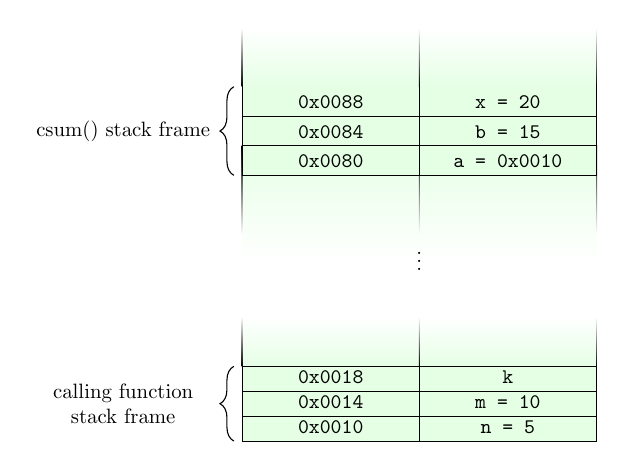
\begin{tikzpicture}[auto,scale=.75,transform shape,every node/.style={text centered}]

%\draw[path fading=north] (0,15.5) -- (0, 18.5);

\draw[fill=green!10!white] (0, 0) rectangle (3, 1.2em);
\node [above] (a1) at (1.5,0) {\texttt{0x0010}};
\draw[fill=green!10!white] (3, 0) rectangle (6, 1.2em);
\node [above] (a2) at (4.5,0) {\texttt{n = 5}};

\draw[fill=green!10!white] (0, 0+1.2em) rectangle (3, 2.4em);
\node [above] (b1) at (1.5,0+1.2em) {\texttt{0x0014}};
\draw[fill=green!10!white] (3, 0+1.2em) rectangle (6, 2.4em);
\node [above] (b2) at (4.5,0+1.2em) {\texttt{m = 10}};

\draw[fill=green!10!white] (0, 0+2.4em) rectangle (3, 3.6em);
\node [above] (b1) at (1.5,0+2.4em) {\texttt{0x0018}};
\draw[fill=green!10!white] (3, 0+2.4em) rectangle (6, 3.6em);
\node [above] (b2) at (4.5,0+2.4em) {\texttt{k}};

\path [top color=white, bottom color=green!10!white] (0,3.625em) rectangle (6,6em);

\fill [top color=white, bottom color=black] (-0.0075,3.6em) rectangle (.02em,6em);
\fill [top color=white, bottom color=black] (5.9925,3.6em) rectangle (6.0075,6em);
\fill [top color=white, bottom color=black] (2.9925,3.6em) rectangle (3.0075,6em);
      
%\draw[top color=white,
%      bottom color=green!10!white]
% (0,3.6em) rectangle (6,6em);
 
%\draw[bottom color=transparent!0,top color=transparent!100] (0,3.6em) -- (0,6em);
%\draw[] (6cm,3.6em) -- (6cm,6em);

%\draw[dashed] (0, 5) -- (6, 5);
%\node [above] (mainvar) at (3,5) {return address, value (\mintinline{c}{0})};
%\draw[dashed] (0, 6) -- (6, 6);
%\node [above] (mainvar2) at (3,6) {local variables \mintinline{c}{n, m, ave}};
\draw [decorate,decoration={brace,amplitude=5pt},xshift=-4pt,yshift=0pt] (0, 0) -- (0, 3.6em) node [text width=3cm,align=center,black,midway,xshift=-.25cm]  {calling function stack frame};


\path [top color=green!10!white, bottom color=white] (0,3) rectangle (6,5);
\fill [top color=black, bottom color=white] (-0.0075,3.5) rectangle (.01,5);
\fill [top color=black, bottom color=white] (2.9925,3.5) rectangle (3.01,5);
\fill [top color=black, bottom color=white] (5.9925,3.5) rectangle (6.01,5);

\draw[fill=green!10!white] (0, 4.5) rectangle (3, 5);
\node [above] (aa1) at (1.5,4.5) {\texttt{0x0080}};
\draw[fill=green!10!white] (3, 4.5) rectangle (6, 5);
\node [above] (aa2) at (4.5,4.5) {\texttt{a = 0x0010}};

\draw[fill=green!10!white] (0, 5) rectangle (3, 5.5);
\node [above] (bb1) at (1.5,5) {\texttt{0x0084}};
\draw[fill=green!10!white] (3, 5) rectangle (6, 5.5);
\node [above] (bb2) at (4.5,5) {\texttt{b = 15}};

\draw[fill=green!10!white] (0, 5.5) rectangle (3, 6);
\node [above] (cc1) at (1.5,5.5) {\texttt{0x0088}};
\draw[fill=green!10!white] (3, 5.5) rectangle (6, 6);
\node [above] (cc2) at (4.5,5.5) {\texttt{x = 20}};

\draw [decorate,decoration={brace,amplitude=5pt},xshift=-4pt,yshift=0pt] (0, 4.5) -- (0, 6) node [text width=3cm,align=center,black,midway,xshift=-.25cm]  {\mintinline{c}{sum()} stack frame};

\node (dots) at (3, 3.15) {$\vdots$};

\path [top color=white, bottom color=green!10!white] (0,6.01) rectangle (6,7);

\fill [top color=white, bottom color=black] (-0.00725,6) rectangle (.0075,7);
\fill [top color=white, bottom color=black] (5.9925,6) rectangle (6.0075,7);
\fill [top color=white, bottom color=black] (2.9925,6) rectangle (3.0075,7);


\end{tikzpicture}
}~~~~\subfigure[The change to the variable \mintinline{c}{a} in the \mintinline{c}{sum()}
function actually changes what the variable \mintinline{c}{a} \emph{references}.  That is, the original
variable \mintinline{c}{n}.]{

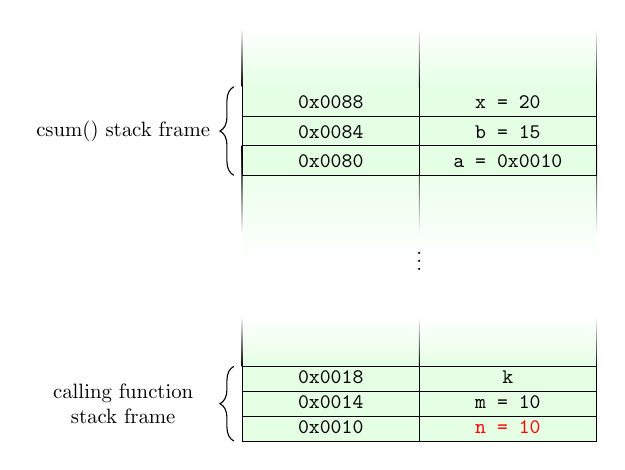
\begin{tikzpicture}[auto,scale=.75,transform shape,every node/.style={text centered}]

%\draw[path fading=north] (0,15.5) -- (0, 18.5);

\draw[fill=green!10!white] (0, 0) rectangle (3, 1.2em);
\node [above] (a1) at (1.5,0) {\texttt{0x0010}};
\draw[fill=green!10!white] (3, 0) rectangle (6, 1.2em);
\node [above] (a2) at (4.5,0) {\color{red}{\texttt{n = 10}}};

\draw[fill=green!10!white] (0, 0+1.2em) rectangle (3, 2.4em);
\node [above] (b1) at (1.5,0+1.2em) {\texttt{0x0014}};
\draw[fill=green!10!white] (3, 0+1.2em) rectangle (6, 2.4em);
\node [above] (b2) at (4.5,0+1.2em) {\texttt{m = 10}};

\draw[fill=green!10!white] (0, 0+2.4em) rectangle (3, 3.6em);
\node [above] (b1) at (1.5,0+2.4em) {\texttt{0x0018}};
\draw[fill=green!10!white] (3, 0+2.4em) rectangle (6, 3.6em);
\node [above] (b2) at (4.5,0+2.4em) {\texttt{k}};

\path [top color=white, bottom color=green!10!white] (0,3.625em) rectangle (6,6em);

\fill [top color=white, bottom color=black] (-0.0075,3.6em) rectangle (.02em,6em);
\fill [top color=white, bottom color=black] (5.9925,3.6em) rectangle (6.0075,6em);
\fill [top color=white, bottom color=black] (2.9925,3.6em) rectangle (3.0075,6em);
      
%\draw[top color=white,
%      bottom color=green!10!white]
% (0,3.6em) rectangle (6,6em);
 
%\draw[bottom color=transparent!0,top color=transparent!100] (0,3.6em) -- (0,6em);
%\draw[] (6cm,3.6em) -- (6cm,6em);

%\draw[dashed] (0, 5) -- (6, 5);
%\node [above] (mainvar) at (3,5) {return address, value (\mintinline{c}{0})};
%\draw[dashed] (0, 6) -- (6, 6);
%\node [above] (mainvar2) at (3,6) {local variables \mintinline{c}{n, m, ave}};
\draw [decorate,decoration={brace,amplitude=5pt},xshift=-4pt,yshift=0pt] (0, 0) -- (0, 3.6em) node [text width=3cm,align=center,black,midway,xshift=-.25cm]  {calling function stack frame};


\path [top color=green!10!white, bottom color=white] (0,3) rectangle (6,5);
\fill [top color=black, bottom color=white] (-0.0075,3.5) rectangle (.01,5);
\fill [top color=black, bottom color=white] (2.9925,3.5) rectangle (3.01,5);
\fill [top color=black, bottom color=white] (5.9925,3.5) rectangle (6.01,5);

\draw[fill=green!10!white] (0, 4.5) rectangle (3, 5);
\node [above] (aa1) at (1.5,4.5) {\texttt{0x0080}};
\draw[fill=green!10!white] (3, 4.5) rectangle (6, 5);
\node [above] (aa2) at (4.5,4.5) { \texttt{a = 0x0010}};

\draw[fill=green!10!white] (0, 5) rectangle (3, 5.5);
\node [above] (bb1) at (1.5,5) {\texttt{0x0084}};
\draw[fill=green!10!white] (3, 5) rectangle (6, 5.5);
\node [above] (bb2) at (4.5,5) {\texttt{b = 15}};

\draw[fill=green!10!white] (0, 5.5) rectangle (3, 6);
\node [above] (cc1) at (1.5,5.5) {\texttt{0x0088}};
\draw[fill=green!10!white] (3, 5.5) rectangle (6, 6);
\node [above] (cc2) at (4.5,5.5) {\texttt{x = 20}};

\draw [decorate,decoration={brace,amplitude=5pt},xshift=-4pt,yshift=0pt] (0, 4.5) -- (0, 6) node [text width=3cm,align=center,black,midway,xshift=-.25cm]  {\mintinline{c}{sum()} stack frame};

\node (dots) at (3, 3.15) {$\vdots$};

\path [top color=white, bottom color=green!10!white] (0,6.01) rectangle (6,7);

\fill [top color=white, bottom color=black] (-0.00725,6) rectangle (.0075,7);
\fill [top color=white, bottom color=black] (5.9925,6) rectangle (6.0075,7);
\fill [top color=white, bottom color=black] (2.9925,6) rectangle (3.0075,7);


\end{tikzpicture}

}

\subfigure[When the \mintinline{c}{sum()} function finishes execution, its stack frame
is removed and the variables \mintinline{c}{a}, \mintinline{c}{b}, and \mintinline{c}{x} are
no longer valid.  The return value 20 is stored in another return value location.]{


\begin{tikzpicture}[auto,scale=.75,transform shape,every node/.style={text centered}]

%\draw[path fading=north] (0,15.5) -- (0, 18.5);

\draw[fill=green!10!white] (0, 0) rectangle (3, 1.2em);
\node [above] (a1) at (1.5,0) {\texttt{0x0010}};
\draw[fill=green!10!white] (3, 0) rectangle (6, 1.2em);
\node [above] (a2) at (4.5,0) {\texttt{n = 10}};

\draw[fill=green!10!white] (0, 0+1.2em) rectangle (3, 2.4em);
\node [above] (b1) at (1.5,0+1.2em) {\texttt{0x0014}};
\draw[fill=green!10!white] (3, 0+1.2em) rectangle (6, 2.4em);
\node [above] (b2) at (4.5,0+1.2em) {\texttt{m = 10}};

\draw[fill=green!10!white] (0, 0+2.4em) rectangle (3, 3.6em);
\node [above] (b1) at (1.5,0+2.4em) {\texttt{0x0018}};
\draw[fill=green!10!white] (3, 0+2.4em) rectangle (6, 3.6em);
\node [above] (b2) at (4.5,0+2.4em) {\color{black}{\texttt{k}}};

\path [top color=white, bottom color=green!10!white] (0,3.625em) rectangle (6,6em);

\fill [top color=white, bottom color=black] (-0.0075,3.6em) rectangle (.02em,6em);
\fill [top color=white, bottom color=black] (5.9925,3.6em) rectangle (6.0075,6em);
\fill [top color=white, bottom color=black] (2.9925,3.6em) rectangle (3.0075,6em);
      
%\draw[top color=white,
%      bottom color=green!10!white]
% (0,3.6em) rectangle (6,6em);
 
%\draw[bottom color=transparent!0,top color=transparent!100] (0,3.6em) -- (0,6em);
%\draw[] (6cm,3.6em) -- (6cm,6em);

%\draw[dashed] (0, 5) -- (6, 5);
%\node [above] (mainvar) at (3,5) {return address, value (\mintinline{c}{0})};
%\draw[dashed] (0, 6) -- (6, 6);
%\node [above] (mainvar2) at (3,6) {local variables \mintinline{c}{n, m, ave}};
\draw [decorate,decoration={brace,amplitude=5pt},xshift=-4pt,yshift=0pt] (0, 0) -- (0, 3.6em) node [text width=3cm,align=center,black,midway,xshift=-.25cm]  {calling function stack frame};


\path [top color=green!10!white, bottom color=white] (0,3) rectangle (6,5);
\fill [top color=black, bottom color=white] (-0.0075,3.5) rectangle (.01,5);
\fill [top color=black, bottom color=white] (2.9925,3.5) rectangle (3.01,5);
\fill [top color=black, bottom color=white] (5.9925,3.5) rectangle (6.01,5);

\draw[fill=green!10!white] (0, 4.5) rectangle (3, 5);
\node [above] (aa1) at (1.5,4.5) {\texttt{0x0080}};
\draw[fill=green!10!white] (3, 4.5) rectangle (6, 5);
\node [above] (aa2) at (4.5,4.5) {\texttt{a = 0x0010}};

\draw[fill=green!10!white] (0, 5) rectangle (3, 5.5);
\node [above] (bb1) at (1.5,5) {\texttt{0x0084}};
\draw[fill=green!10!white] (3, 5) rectangle (6, 5.5);
\node [above] (bb2) at (4.5,5) {\texttt{b = 15}};

\draw[fill=green!10!white] (0, 5.5) rectangle (3, 6);
\node [above] (cc1) at (1.5,5.5) {\texttt{0x0088}};
\draw[fill=green!10!white] (3, 5.5) rectangle (6, 6);
\node [above] (cc2) at (4.5,5.5) {\texttt{x = 20}};

%cross outs: 
\draw[pattern=north west lines, pattern color=blue!50!white] (0,4.5) rectangle (6,6);


\draw [decorate,decoration={brace,amplitude=5pt},xshift=-4pt,yshift=0pt] (0, 4.5) -- (0, 6) node [text width=3cm,align=center,black,midway,xshift=-.25cm]  {\mintinline{c}{sum()} stack frame};

\node (dots) at (3, 3.15) {$\vdots$};

\path [top color=white, bottom color=green!10!white] (0,6.01) rectangle (6,7);

\fill [top color=white, bottom color=black] (-0.00725,6) rectangle (.0075,7);
\fill [top color=white, bottom color=black] (5.9925,6) rectangle (6.0075,7);
\fill [top color=white, bottom color=black] (2.9925,6) rectangle (3.0075,7);


\end{tikzpicture}

}~~~~~\subfigure[The returned value is stored in the variable \mintinline{c}{k} and
the value in the variable \mintinline{c}{n} has now changed.]{


\begin{tikzpicture}[auto,scale=.75,transform shape,every node/.style={text centered}]

%\draw[path fading=north] (0,15.5) -- (0, 18.5);

\draw[fill=green!10!white] (0, 0) rectangle (3, 1.2em);
\node [above] (a1) at (1.5,0) {\texttt{0x0010}};
\draw[fill=green!10!white] (3, 0) rectangle (6, 1.2em);
\node [above] (a2) at (4.5,0) {\texttt{n = 10}};

\draw[fill=green!10!white] (0, 0+1.2em) rectangle (3, 2.4em);
\node [above] (b1) at (1.5,0+1.2em) {\texttt{0x0014}};
\draw[fill=green!10!white] (3, 0+1.2em) rectangle (6, 2.4em);
\node [above] (b2) at (4.5,0+1.2em) {\texttt{m = 10}};

\draw[fill=green!10!white] (0, 0+2.4em) rectangle (3, 3.6em);
\node [above] (b1) at (1.5,0+2.4em) {\texttt{0x0018}};
\draw[fill=green!10!white] (3, 0+2.4em) rectangle (6, 3.6em);
\node [above] (b2) at (4.5,0+2.4em) {\color{red}{\texttt{k = 20}}};

\path [top color=white, bottom color=green!10!white] (0,3.625em) rectangle (6,6em);

\fill [top color=white, bottom color=black] (-0.0075,3.6em) rectangle (.02em,6em);
\fill [top color=white, bottom color=black] (5.9925,3.6em) rectangle (6.0075,6em);
\fill [top color=white, bottom color=black] (2.9925,3.6em) rectangle (3.0075,6em);
      
%\draw[top color=white,
%      bottom color=green!10!white]
% (0,3.6em) rectangle (6,6em);
 
%\draw[bottom color=transparent!0,top color=transparent!100] (0,3.6em) -- (0,6em);
%\draw[] (6cm,3.6em) -- (6cm,6em);

%\draw[dashed] (0, 5) -- (6, 5);
%\node [above] (mainvar) at (3,5) {return address, value (\mintinline{c}{0})};
%\draw[dashed] (0, 6) -- (6, 6);
%\node [above] (mainvar2) at (3,6) {local variables \mintinline{c}{n, m, ave}};
\draw [decorate,decoration={brace,amplitude=5pt},xshift=-4pt,yshift=0pt] (0, 0) -- (0, 3.6em) node [text width=3cm,align=center,black,midway,xshift=-.25cm]  {calling function stack frame};


\path [top color=green!10!white, bottom color=white] (0,3) rectangle (6,5);
\fill [top color=black, bottom color=white] (-0.0075,3.5) rectangle (.01,5);
\fill [top color=black, bottom color=white] (2.9925,3.5) rectangle (3.01,5);
\fill [top color=black, bottom color=white] (5.9925,3.5) rectangle (6.01,5);

\draw[fill=green!10!white] (0, 4.5) rectangle (3, 5);
\node [above] (aa1) at (1.5,4.5) {\texttt{0x0080}};
\draw[fill=green!10!white] (3, 4.5) rectangle (6, 5);
\node [above] (aa2) at (4.5,4.5) {\texttt{a = 0x0010}};

\draw[fill=green!10!white] (0, 5) rectangle (3, 5.5);
\node [above] (bb1) at (1.5,5) {\texttt{0x0084}};
\draw[fill=green!10!white] (3, 5) rectangle (6, 5.5);
\node [above] (bb2) at (4.5,5) {\texttt{b = 15}};

\draw[fill=green!10!white] (0, 5.5) rectangle (3, 6);
\node [above] (cc1) at (1.5,5.5) {\texttt{0x0088}};
\draw[fill=green!10!white] (3, 5.5) rectangle (6, 6);
\node [above] (cc2) at (4.5,5.5) {\texttt{x = 20}};

%cross outs: 
\draw[pattern=north west lines, pattern color=blue!50!white] (0,4.5) rectangle (6,6);


\draw [decorate,decoration={brace,amplitude=5pt},xshift=-4pt,yshift=0pt] (0, 4.5) -- (0, 6) node [text width=3cm,align=center,black,midway,xshift=-.25cm]  {\mintinline{c}{sum()} stack frame};

\node (dots) at (3, 3.15) {$\vdots$};

\path [top color=white, bottom color=green!10!white] (0,6.01) rectangle (6,7);

\fill [top color=white, bottom color=black] (-0.00725,6) rectangle (.0075,7);
\fill [top color=white, bottom color=black] (5.9925,6) rectangle (6.0075,7);
\fill [top color=white, bottom color=black] (2.9925,6) rectangle (3.0075,7);


\end{tikzpicture}

}

\caption[Demonstration of Pass By Reference]{Demonstration of Pass By Reference.  
Passing variables by reference means that the \emph{memory address} of the variables
are provided to the function.  The function is able to make changes to the original variable
because it knows where it is stored.}
\label{figure:PassByReference}

\end{figure}




%\end{document}


Whether or not a variable is passed by value or by reference depends
on the language, type of variable, and the syntax used.  

\section{Other Issues}

\subsection{Functions as Entities}

In programming languages, any entity that can be stored in a variable or
passed as an argument to a function or returned as a value from a function
is referred to as a ``first-class citizen.''  \index{first-class citizen}
Numerical values for example are
usually first-class  citizens as they can be stored in variables and passed 
to functions.

\emph{Functional Programming} \index{functional programming}
is a programming language paradigm in
which functions themselves are first-class citizens.  That is, functions can
be assigned to variables, functions can be passed to other functions as 
arguments, and functions can even return functions as a result.  This is
done as a matter of course in functional programming languages such as
Haskell and Clojure, but many programming languages contain some 
functional aspects.

For example, some languages support the same concept by using function 
\emph{pointers} which are essentially references to where the function is stored in memory.
As a memory location is essentially a number, it can be passed around in
functions and be stored in a variable.  Purists would argue that this is
not sufficient to call a function a ``first-class citizen'' in such a language.
They may argue that a language must be able to create new functions
at runtime for it to be considered a language in which functions are 
``true'' first-class citizens.

In any case, there are several advantages to being able to pass functions
around as arguments or store them in variables.  Passing a function
to another function as an argument gives you the ability to provide a
\gls{callback}.  A \index{callback} callback is simply a function that gets passed to another
function as an argument.  The idea is that the function that receives
the callback will execute or ``call back'' the passed function at some
point.

Using callbacks enables us to program a ``generic'' function that 
provides some generalized functionality.  Then more specific behavior
can be be implemented in the callback function.  For example, we 
could create a generic \emph{sort} function that sorts elements in a
collection.  We could make the sort function generic so that it could
sort any type of data: numbers, strings, objects, etc.  A callback would
provide more specific behavior on how to \emph{order} individual
elements in the sorted array.  

As another example, consider \gls{guiLabel} Programming in which we
want to design a user interface.  In particular, we may be able to create
a button element in our interface.  We need to be able to specify what 
happens when the user clicks the button.  This could be achieved by
passing in a function as a callback to ``register'' it with the click ``event.''

%Closures? https://en.wikipedia.org/wiki/Closure_(computer_programming)

A related issue is \glspl{anonymous function} (also known as 
\glspl{lambda expression}).  Typically, we simply 
want to create a function so that we can pass it as a callback to another 
function.  We may have no intention of actually calling this function directly
as it may not be of much use other than passing it as a callback.  Some 
languages allow you to define a function ``inline'' without an identifier 
so that it can be passed to another function.  Since the function has no
name and cannot be invoked by other sections of the code (other than
the function we passed it to), it is known as an anonymous function.

\subsection{Function Overloading}
\label{subsection:functionOverloading}
\label{function overloading}

Some languages do not allow you to define more than one function with
the same name in the same scope.  This is to prevent ambiguity in the
code.  When you write code to invoke a function and there are several
functions with that name, which one are you actually calling?  

Some languages \emph{do} allow you to define multiple functions
with the same name as long as they differ in either the number (also
called \emph{arity}) or 
type of parameters.  For example, you could define two absolute
value, $|x|$ functions with the same name, but one of them takes a floating
point number while the other takes an integer as its parameter.  This
is known as \gls{function overloading} because you are ``overloading''
the code by defining multiple functions with the same name.

The ambiguity problem is solved by requiring that each function with the
same name differs in their parameters.  If you invoke the absolute
value function and pass it a floating point number, clearly you meant 
to call the first version.  If you passed it an integer, it is clear that you
intended to invoke the second version.  Depending on the type and
number of arguments you pass to a function, the compiler or 
interpreter is able to determine \emph{which} version you intend
to call and is able to make the right function call.  This process is
known as \gls{static dispatch}.

In a language without function overloading, we would be forced to
use different names for functions that perform the same operation
but on different types.  

\subsection{Variable Argument Functions}
\index{variable argument function|see {vararg function}}
\index{vararg function}

Many languages allow you to define special functions that take
a \emph{variable number} of parameters.  Often they are referred
to as ``vararg'' (short for variable argument) functions.  The syntax
for doing so varies as does how you can write a function to operate
on a variable number of arguments (usually through some array or
collection data structure).

The standard \mintinline{text}{printf} (print formatted) function found
in many languages is a good example of a vararg function.  The
\mintinline{text}{printf} function allows you to use one function to
print any number of variables or values.  Without a vararg function,
you would have to implement a \mintinline{text}{printf} version for
no arguments, 1 argument, 2 arguments, etc.  Even then, you
would only be able to support up to $n$ arguments for as many 
functions as you defined.  By using a vararg function, we can write
a single function that operates on all of these possibilities.  It
is import to note, a vararg function is \emph{not} an example of
function overloading.  There is still only \emph{one} function defined, 
it just takes a variable number of arguments.

\subsection{Optional Parameters \& Default Values}
\label{subsection:optionalParameters}
\index{optional parameters}

Suppose that you define a function which has, say, three 
parameters.  Now suppose you invoke the function but only
provide it 2 of the 3 arguments that it expects.  Some languages
would not allow this and it would be considered a syntax or
runtime error.  Yet other languages may have very complex 
rules about what happens when an argument is omitted.  Some
languages allow you to omit some arguments when calling functions
as a feature of the language.  That is, the parameters to a function
are \emph{optional}.  

When a language allows parameters to be optional, it usually also
allows you to define \emph{default values} to the parameters if
the calling function does not provide them.   If a user calls the
function without specifying a parameter, it takes on the default
value.  Alternatively, the default could be a non-value like ``null''
or ``undefined.''  Inside the function you could implement logic that 
determined whether or not a parameter was passed to the function
and alter the behavior of the function accordingly.  

